\documentclass[12]{article}
\usepackage[margin=1.0in]{geometry}
\usepackage[utf8]{inputenc}
\usepackage{titlesec}
\usepackage{physics}
\usepackage{graphicx}
\usepackage{siunitx}
\usepackage{cancel}
\usepackage{amsmath}
\usepackage{textcomp}
\usepackage{gensymb}
\usepackage{natbib}
\usepackage{bm}
\usepackage{setspace}
\usepackage[version=4]{mhchem}

\titleformat*{\subsection}{\normalfont\fontfamily{phv}}
%\titleformat*{\subsection}[runin]{}{}{}{}[]
  \titleformat{\subsection}[runin]{\normalfont\bfseries}{\thesubsection.}{3pt}{}
  \titleformat{\subsubsection}[runin]{\normalfont\bfseries}{\thesubsubsection.}{3pt}{}

\title{{\textsc{\Large Antarctic Radiative and Temperature responses to a doubling of $\text{CO}_2$}}}
\author{\textsc{}}
\doublespacing

\begin{document}
\maketitle
\thispagestyle{empty}

\setlength{\leftskip}{1.1cm}
\setlength{\rightskip}{1.1cm}


\bigskip
\bigskip

{\textsc{Abstract.} }Greenhouse gases (GHGs), such as \ce{CO2}, impact global and local outgoing longwave radiation (OLR). The Antarctic is known for its a strong near-surface temperature inversion, where the addition of GHGs can lead to increased OLR during all but the winter months.  Here we develop a radiative-advective-turbulent single-column model based on observed temperatures at the South Pole and timestep it forward under different \ce{CO_2} concentrations. Despite this increase in OLR, we confirm that surface temperatures in the Antarctic warm as \ce{CO_2} emissions increase. Therefore, we look at the relationship between the surface greenhouse effect and surface temperature responses, ******. We look at the surface greenhouse effect as a function of both the Planck function and a simplified effective bandwidth of \ce{CO2} 

% Target: GRL-length paper? 4 figures + 4000 words, <150 words in abstract

%% Possible outline with figures:

% Introduction

% Radiative calculations (without forward time stepping) - methods + results
% 1) TOA and surface greenhouse effect of CO2 (line plots against CO2)
% 2) explain surface GHE of CO2 as a consequence of F ~ B(\nu,T_S) * l_eff(C) [line plot against CO2 and possibly a scatter plot? not sure.]

% Radiative-advective-turbulent calculations - methods + results (surface exchange + advection + time stepping all need to be documented)
% 3) \Delta T (2xCO2 - 1xCO2) for all months with sub-panels for surface T change

% Discussion 
% 4) predicted surface temperature change (relative to no CO2) compared to radiative-advective-turbulent model calculations (scatter plot)

% Conclusions

\section{Introduction}
\section{Methods}
\subsection{Model Setup}
\section{Results}
\begin{figure}[htb!]
\noindent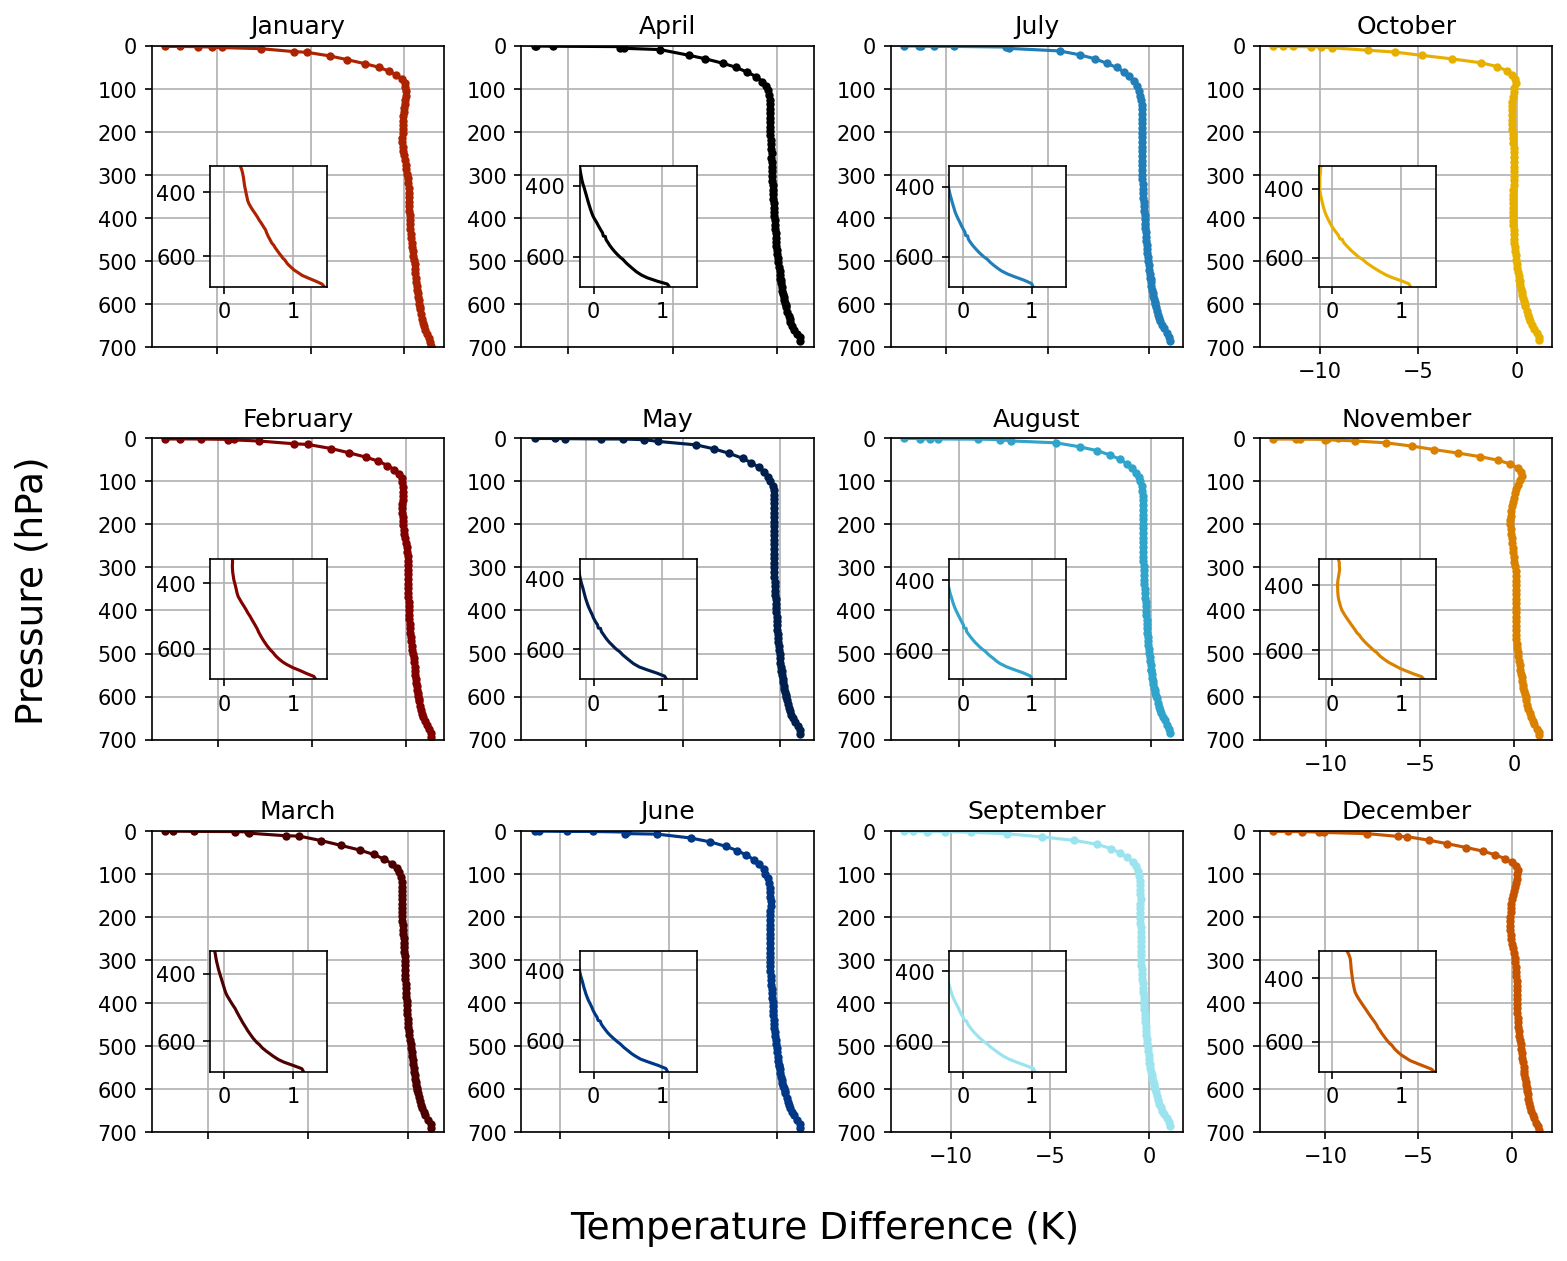
\includegraphics[width=1\textwidth]{figures/temp_dif.png}
\centering
\caption{}
\label{fig:temp_dif}
\end{figure}

\begin{figure}[htb!]
\noindent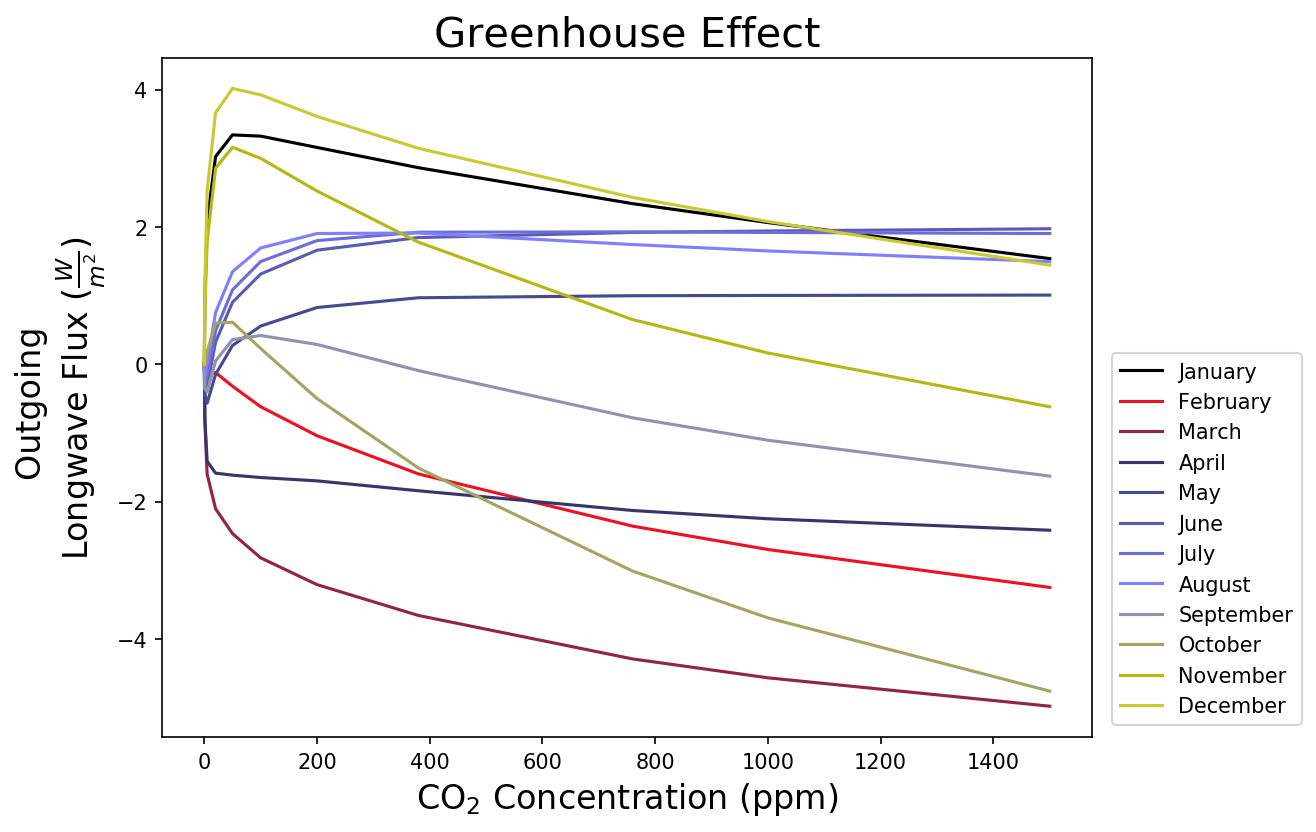
\includegraphics[width=1\textwidth]{figures/GHE.png}
\centering
\caption{}
\label{fig:GHE}
\end{figure}

\begin{figure}[htb!]
\noindent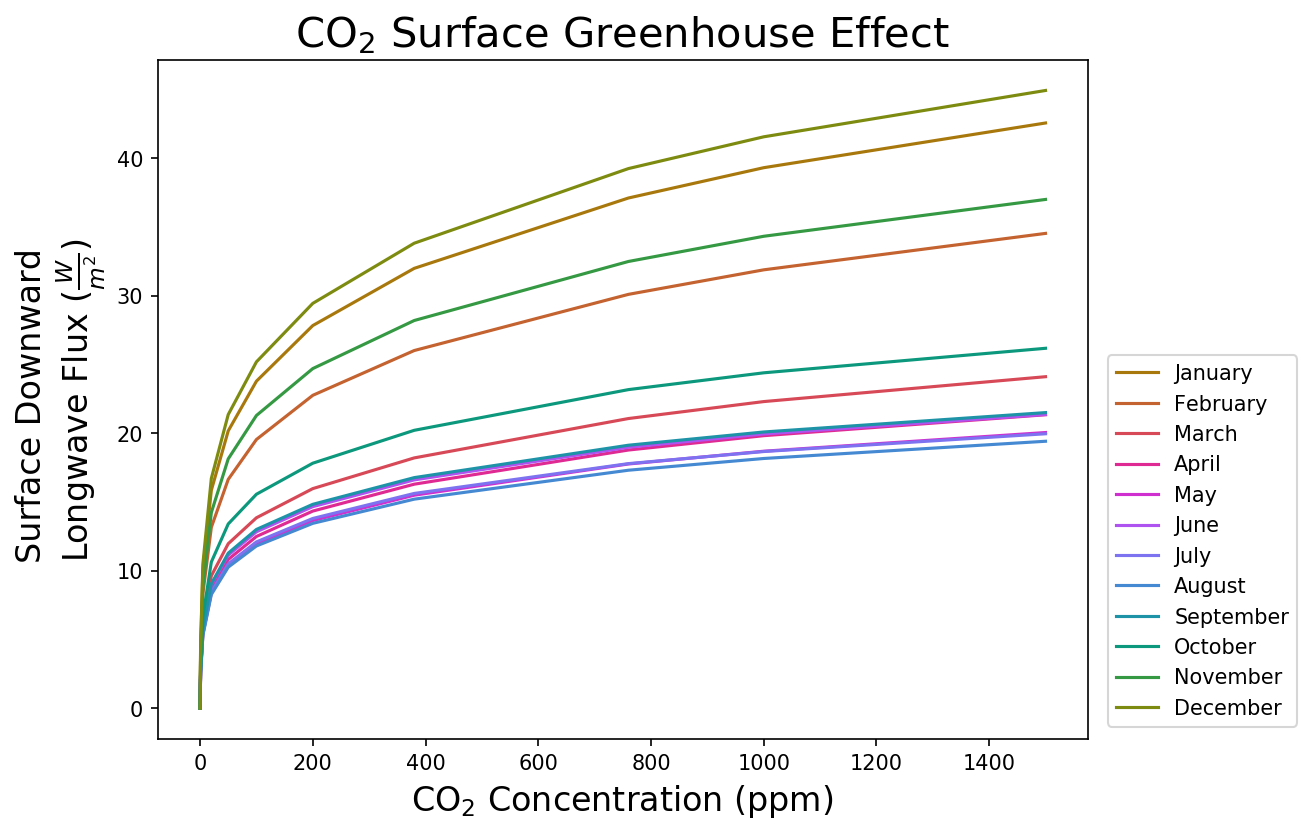
\includegraphics[width=1\textwidth]{figures/sfc_CO2_effect.png}
\centering
\caption{}
\label{fig:sfc_CO2_effect}
\end{figure}

\begin{figure}[htb!]
\noindent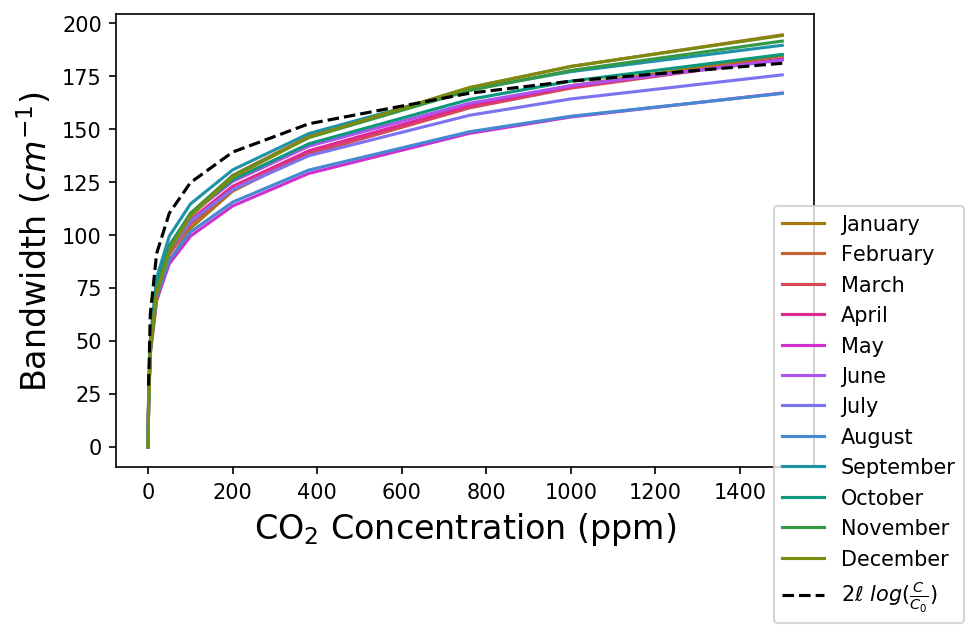
\includegraphics[width=1\textwidth]{figures/sfc_bandwidth.png}
\centering
\caption{}
\label{fig:sfc_bandwidth}
\end{figure}




\subsection{Equilibrium State}
\subsection{Bandwidth Analysis}
\section{Discussion}

\bibliographystyle{apalike}
\bibliography{references.bib}

\end{document}
